\documentclass[11pt]{beamer}
\usetheme{Warsaw}
\usepackage[T1]{fontenc}
\usepackage[utf8]{inputenc}
\usepackage{amsmath}
\usepackage{amsfonts}
\usepackage{amssymb}
\usepackage{graphicx}
\usepackage{setspace}
\usepackage{hyperref}
\author{Chen ZHANG \inst{1,2}}
\title{TPMplt: R Toolkit for Dynamic Materials Modeling}
%\setbeamercovered{transparent} 
%\setbeamertemplate{navigation symbols}{} 
\setbeamertemplate{enumerate items}[default]
\logo{
\includegraphics[width=.15\textwidth]{logo.png}}
\institute[UNI]{\inst{1}Tohoku University, \inst{2}Institute for Material Research $@$ Sendai, Japan\\[2.5ex] {Git URL: \href{https://github.com/CubicZebra/TPMplt}{\color{cyan}\underline{CubicZebra/TPMplt.git}}}}
\date{2018.11.29}
%\subject{} 
\newcommand{\code}[1]{\texttt{#1}}
\AtEndDocument{\begin{frame}{\huge \quad Thanks for your attention.}\end{frame}}
\begin{document}

\begin{frame}
\titlepage
\end{frame}

\begin{frame}
\tableofcontents
\end{frame}

\section{Introduction}
\subsection{Depandencies \& Installations}
\begin{frame}{Depandencies}
\begin{enumerate}
	\item R framework:
    \begin{enumerate}
    	   \item For Windows \& OS X: Install via official installer
        \item For linux: Install r-base as root
    \end{enumerate}
    \item An IDE for R: RStudio, Visual Studio (Windows only), ...
    \item X11 framework:
    \begin{enumerate}
    	   \item For Windows \& OS X: XQuartz via offical installer
        \item For linux: \code{sudo apt-get install xorg openbox libx11-dev libglu1-mesa-dev libfreetype6-dev}
    \end{enumerate}
\end{enumerate}
\end{frame}

\begin{frame}{Installation}
\begin{enumerate}
	\item Version: 0.1.0
	\item License: GPLv3
	\item Installation: 
	\begin{enumerate}
		\item From CRAN (stable): \code{install.packages("TPMplt")}
		\item From Git Repo (Developement): \\
		\qquad \code{if(!"devtools" \%in\% installed.packages())\\ \qquad \qquad install.packages("devtools")}\\
		\qquad \code{devtools::install\_github("CubicZebra/TPMplt")}
	\end{enumerate}
\end{enumerate}
\end{frame}

\subsection{VBT Data Frame}
\begin{frame}{Conventional Data Frame}
    \begin{minipage}[t]{0.5\textwidth}
        \vspace{0pt}
        \begin{itemize}
            \item Including \emph{discrete} and \emph{continous} variables
            \item \emph{\color{red}Discrete} ones copied and aligned in \emph{\color{red}individual columns}
            \item Take \code{iris3} as example $\rightarrow$ \\ {\footnotesize\color{olive}(*note: \code{iris3} is a basic dataset for testing)}
        \end{itemize}
    \end{minipage}%
    \hfill
    \begin{minipage}[t]{0.45\textwidth}
        \vspace{0pt}
        \centering
              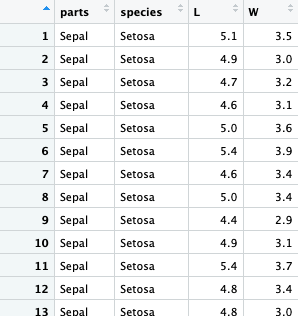
\includegraphics[height=5cm, width=4.5cm]{Fig1.png}
    \end{minipage}
\end{frame}

\begin{frame}{VBT Data Frame}
    \begin{minipage}[t]{0.5\textwidth}
        \vspace{0pt}
        \begin{itemize}
            \item Including \emph{discrete} and \emph{continous} variables
            \item \emph{\color{red}Discrete} ones contained in \emph{\color{red}column names} with specific structure \\ {\footnotesize\color{olive}(*intuitively corresponding most experimental data)}
            \item Take \code{iris3} as example $\rightarrow$
            \item For details: \href{https://CRAN.R-project.org/package=VBTree}{\color{cyan}\underline{VBTree package}}
        \end{itemize}
    \end{minipage}%
    \hfill
    \begin{minipage}[t]{0.45\textwidth}
        \vspace{0pt}
        \centering
              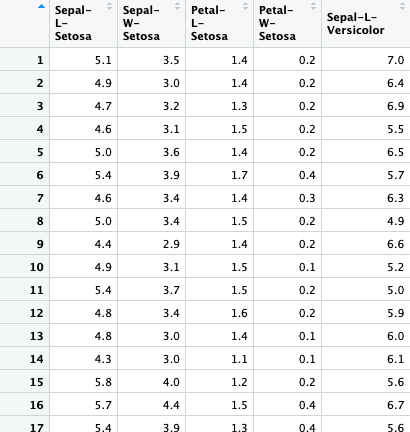
\includegraphics[height=5cm, width=4.5cm]{Fig2.png}
    \end{minipage}
\end{frame}

\subsection{Workflow Overview}
\begin{frame}{Workflow}
\centering
	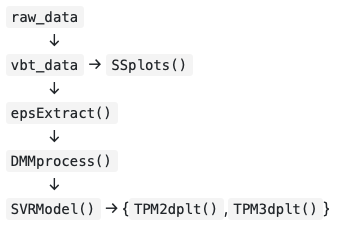
\includegraphics[scale=0.6]{Fig3.png}
\end{frame}

\section{Practical Application}
\subsection{Hot Working Properties for Alloys}
\begin{frame}[t]{Fe{\color{red}13Cr}WCuC}
	\begin{minipage}[t]{1\textwidth}
        \vspace{0pt}
        \begin{itemize}
            \item {\small Summary VBT data frame\\{\scriptsize\color{olive}(32 columns with 4 temperatures * 4 strain rates * \{Strain, Stress\})}}\\
            \singlespacing
            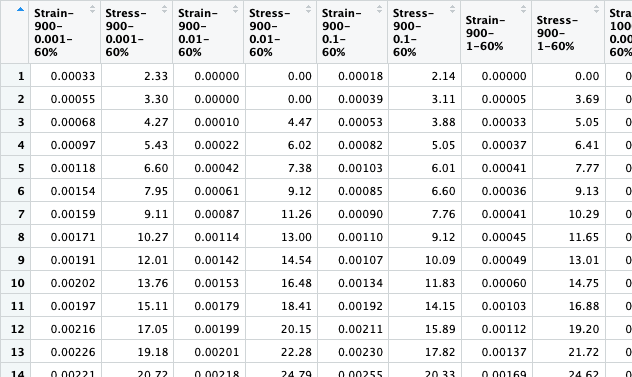
\includegraphics[scale=0.37]{Fig4.png}
        \end{itemize}
    \end{minipage}%
\end{frame}

\begin{frame}[t]{Fe{\color{red}13Cr}WCuC}
	\begin{minipage}[t]{1\textwidth}
        \vspace{0pt}
        \begin{itemize}
            \item {\small Stress-Strain plots grouped by temperature:\\ {\scriptsize\code{R$>$ SSplot(vbt\_data, {\color{red}2}, mfrow=c(2,2))}}}\\
            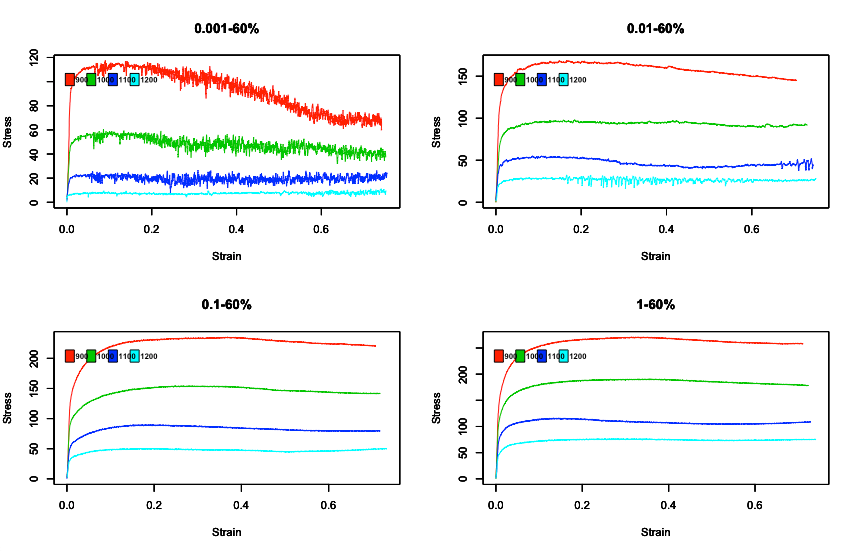
\includegraphics[scale=0.29]{Fig5.png}
        \end{itemize}
    \end{minipage}%
\end{frame}

\begin{frame}[t]{Fe{\color{red}13Cr}WCuC}
	\begin{minipage}[t]{1\textwidth}
        \vspace{0pt}
        \begin{itemize}
            \item {\small Stress-Strain plots grouped by strain rate:\\ {\scriptsize\code{R$>$ SSplot(vbt\_data, {\color{red}3}, mfrow=c(2,2))}}}\\
            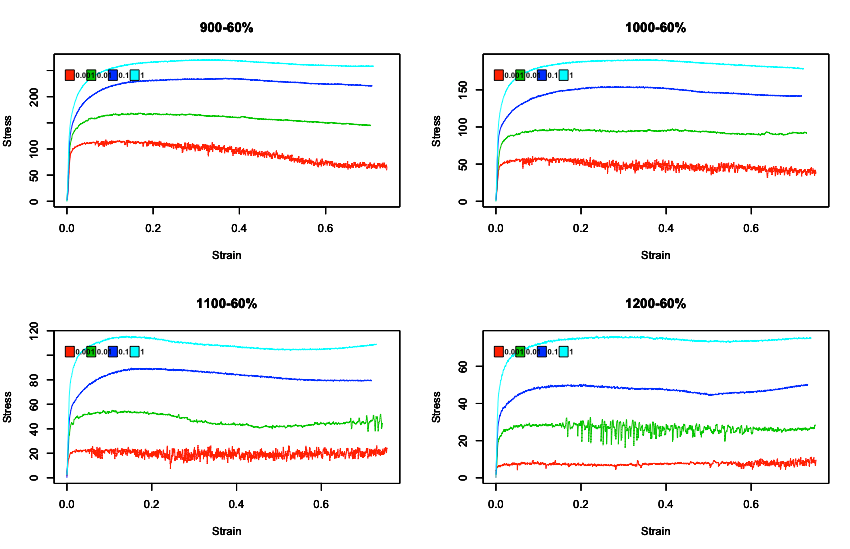
\includegraphics[scale=0.29]{Fig6.png}
        \end{itemize}
    \end{minipage}%
\end{frame}

\begin{frame}[t]{Fe{\color{red}13Cr}WCuC}
	\begin{minipage}[t]{1\textwidth}
        \vspace{0pt}
        \begin{itemize}
            \item {\small Build dynamic materials model (at 0.7 strain):\\
            {\scriptsize\code{R$>$ SRT <- epsExtract(vbt\_data, {\color{red}0.7}, 2, 3)\\
            R$>$ DMM <- DMMprocess(SRT)\\
            R$>$ print(DMM)
            }}
            }\\
            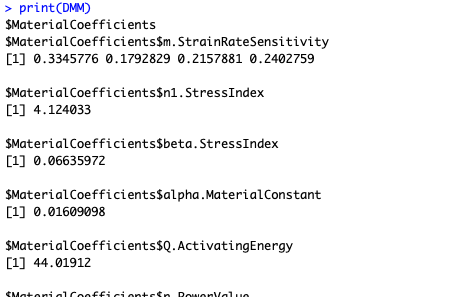
\includegraphics[scale=0.4]{Fig7.png}
        \end{itemize}
    \end{minipage}%
\end{frame}

\begin{frame}[t]{Fe{\color{red}13Cr}WCuC}
	\begin{minipage}[t]{1\textwidth}
        \vspace{0pt}
        \begin{itemize}
            \item {\small Regression and 2d visulization (radial basis kernel (\code{rbf}) in SVM):\\
            {\scriptsize\code{R$>$ SVR <- SVRModel(DMM)\\
            R$>$ TPM2dplt(SVR)
            }}
            }\\
            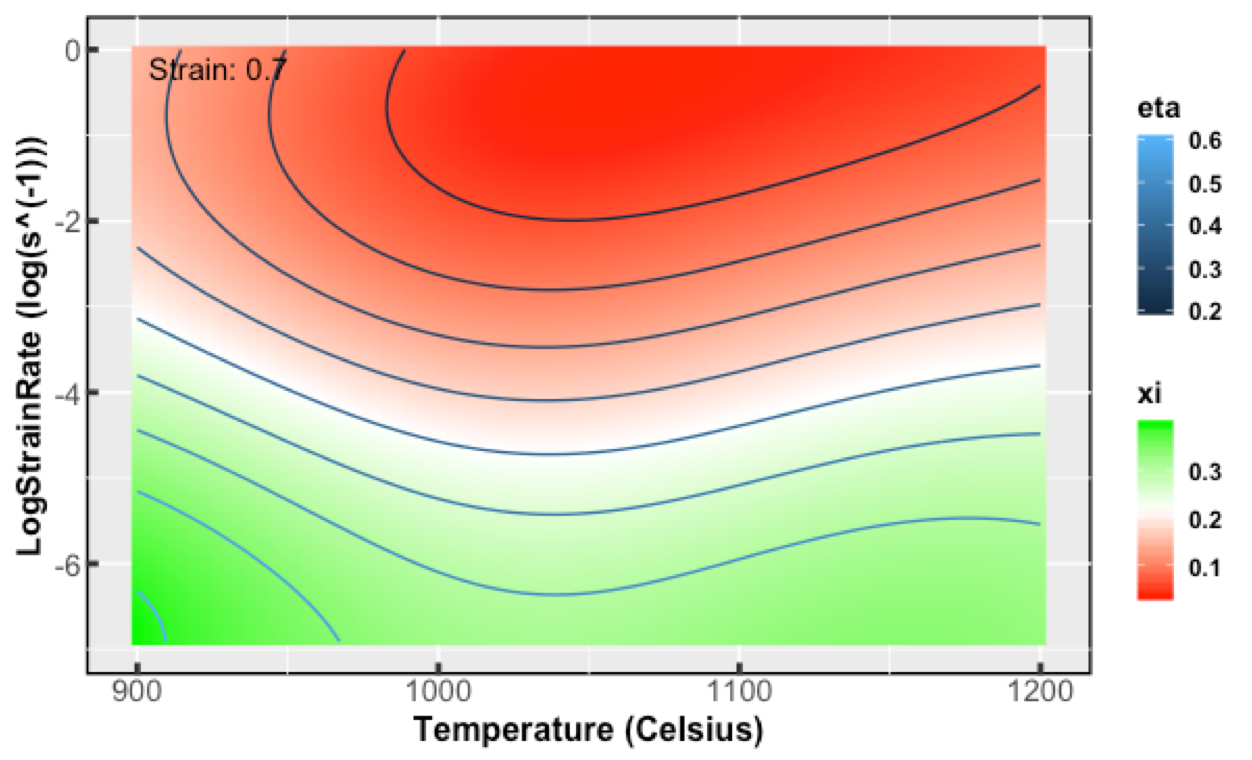
\includegraphics[scale=0.38]{Fig8.png}
        \end{itemize}
    \end{minipage}%
\end{frame}

\begin{frame}[t]{Fe{\color{red}13Cr}WCuC}
	\begin{minipage}[t]{1\textwidth}
        \vspace{0pt}
        \begin{itemize}
            \item {\small 3d visulization:\\
            {\scriptsize\code{R$>$ TPM3dplt(SVR)
            }}
            }\\
            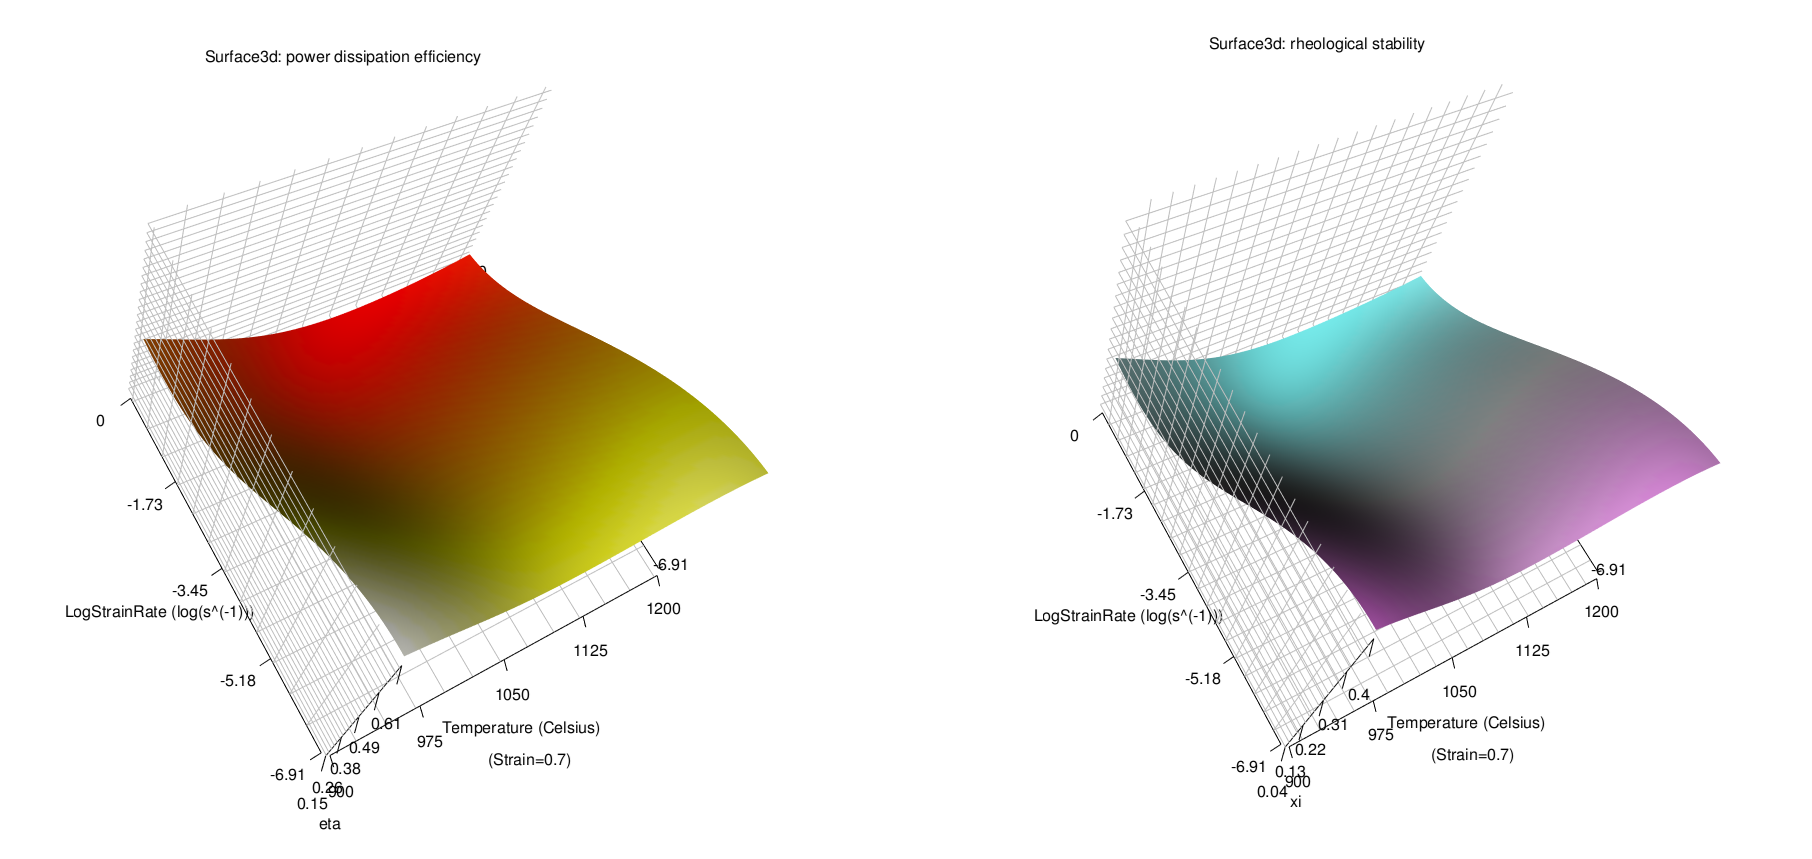
\includegraphics[scale=0.157]{Fig9.png}
        \end{itemize}
    \end{minipage}%
\end{frame}

\begin{frame}{Fe{\color{red}16Cr}WCuC}
	\begin{minipage}[t]{1\textwidth}
        \vspace{0pt}
        \begin{itemize}
        	   \item {\small Similar as workflow of 13Cr}
            \item {\small Sequential plots are available using loop script:\\
            \singlespacing
            {\scriptsize\code{R$>$ seqeps <- seq(0.1, 0.8, 0.1)\\
            R$>$ for (i in 1:8) \{\\
            \qquad + SRT <- epsExtract(vbt\_data, seqeps[i], 2, 3)\\
            \qquad + DMM <- DMMprocess(SRT)\\
            \qquad + PLTbd <- SVRModel(DMM)\\
            \qquad + plt <- TPM2dplt(PLTbd)\\
            \qquad + print(plt)\\
            \qquad + Sys.sleep(5)\\
            \qquad + \}\\
            R$>$ \#Sys.sleep() controls holding time for each plot
            }}
            }\\
        \end{itemize}
    \end{minipage}%
\end{frame}

\begin{frame}[t]{Fe{\color{red}16Cr}WCuC}
	\begin{minipage}[t]{1\textwidth}
        \vspace{0pt}
        \begin{itemize}
            \item {\small Sequential 2d plots:}
            \\
            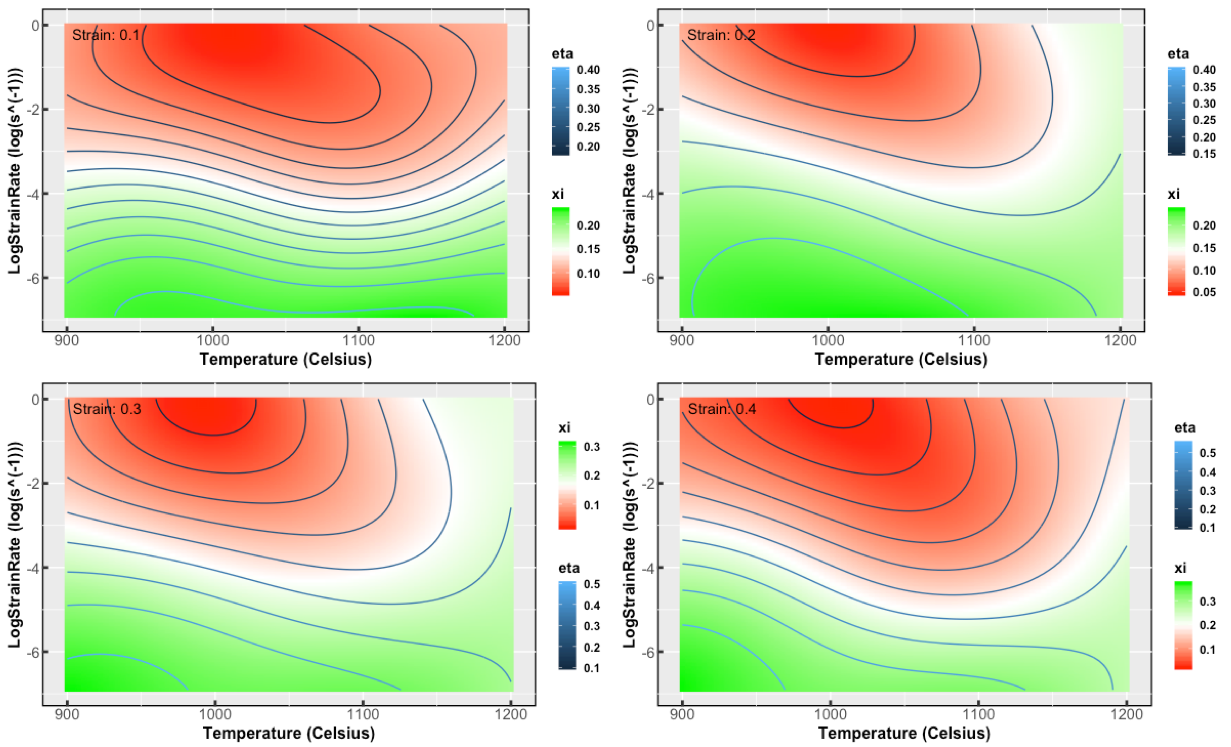
\includegraphics[scale=0.45]{Fig10.png}
        \end{itemize}
    \end{minipage}%
\end{frame}

\begin{frame}[t]{Fe{\color{red}16Cr}WCuC}
	\begin{minipage}[t]{1\textwidth}
        \vspace{0pt}
        \begin{itemize}
            \item {\small Sequential 2d plots:}
            \\
            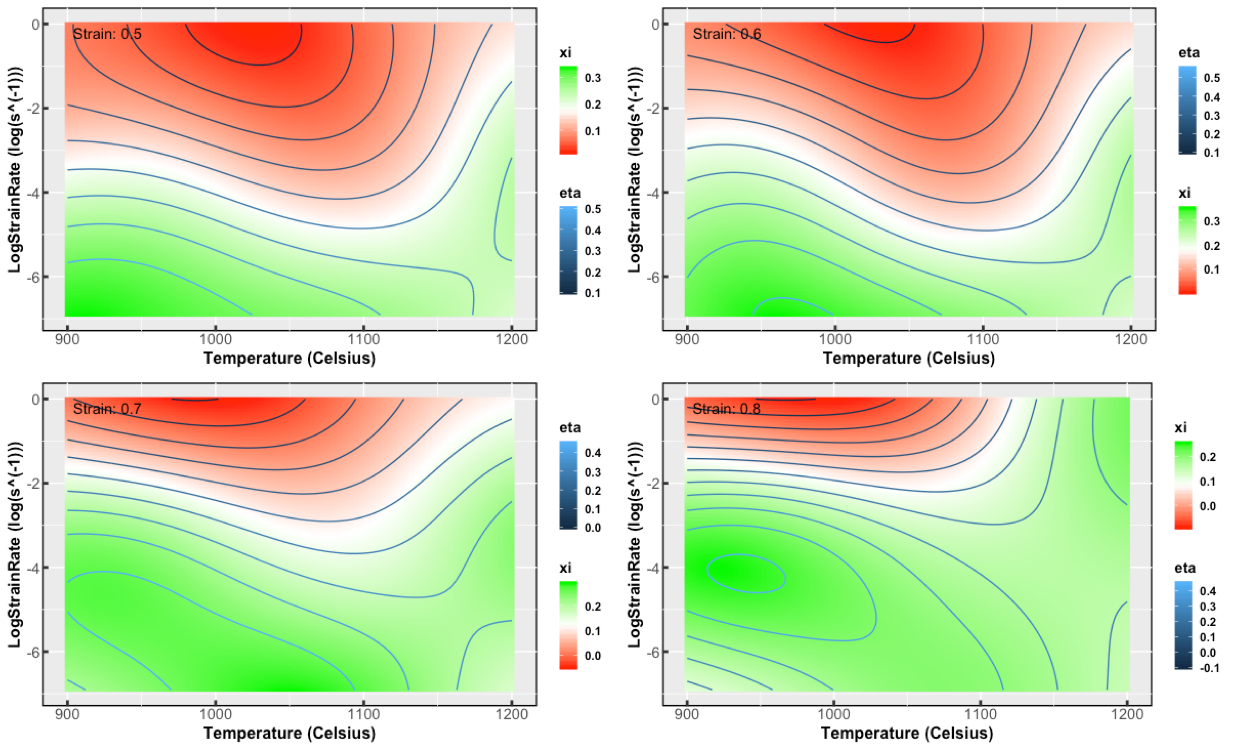
\includegraphics[scale=0.45]{Fig11.png}
        \end{itemize}
    \end{minipage}%
\end{frame}

\begin{frame}[t]{Fe{\color{red}16Cr}WCuC}
	\begin{minipage}[t]{1\textwidth}
        \vspace{0pt}
        \begin{itemize}
            \item {\small 3d plot using 0.7 strain (unstable plan added for plot of $\xi$):}
            \\
            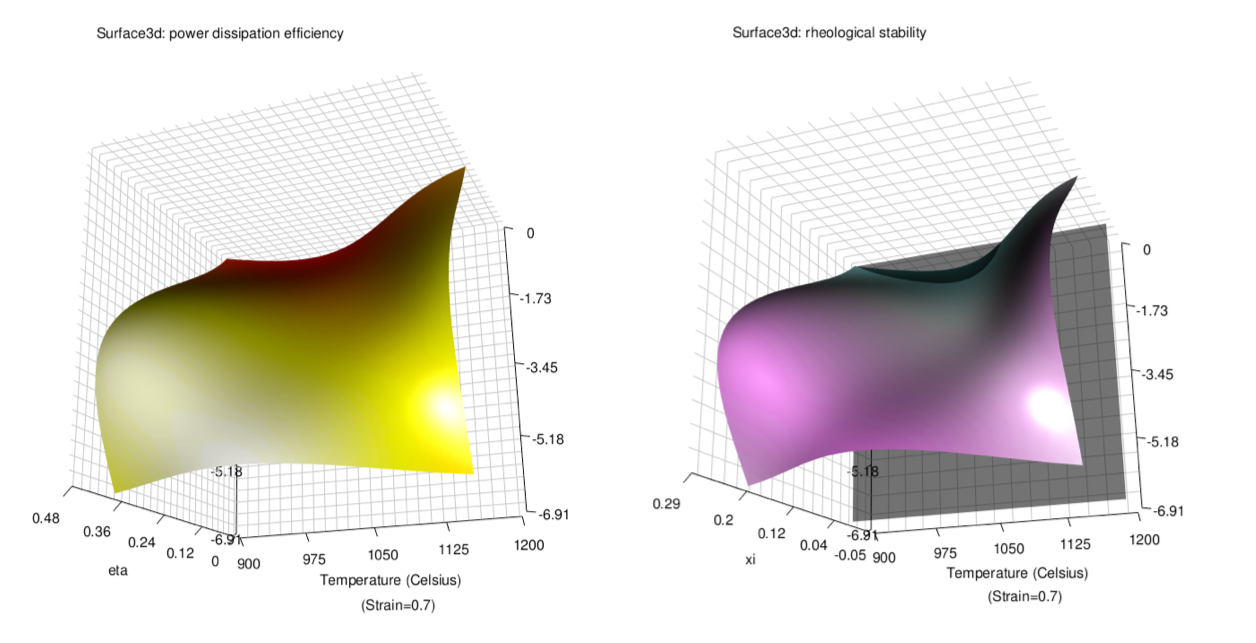
\includegraphics[scale=0.47]{Fig12.png}
        \end{itemize}
    \end{minipage}%
\end{frame}

\section{Under Developement}
\subsection{Insufficiencies \& Solutions}
\begin{frame}{Insufficiencies}
\begin{enumerate}
	\item $\because m \in (0, 1) \therefore \eta = 2m/(1+m) \in (0, 1)$\\ However, some predicted $\eta$ values are still out of range
	\singlespacing
	\item Result of material constant A looks strange, since it's too small in magnitude
	\singlespacing
	\item Values for contours generated by \code{TPM2dplt()}  are invisible
\end{enumerate}
\end{frame}

\begin{frame}{Corresponding Solutions}
\begin{enumerate}
	\item Truncate the $\eta$ using estimator $\tilde{\eta} = (\eta - \eta_{min})/(\eta_{max} - \eta_{min})$
	\singlespacing
	\item Modify related calculations in model-buiding function
	\singlespacing
	\item Updata 2d visualization function with the \code{directlabels} package
\end{enumerate}
\end{frame}

\subsection{Modification for Next Version}
\begin{frame}{Functions to be Updated}
\begin{itemize}
	\item Functions required modification includes:
	\singlespacing
	\begin{enumerate}
		\item \code{DMMprocess()}
		\item \code{SVRModel()}
		\item \code{TPM2dplt()}
	\end{enumerate}
\end{itemize}
\end{frame}

%\begin{frame}{Fig Insert Template}
%    \begin{minipage}{0.5\textwidth}
%        \vspace{0pt}
%        \begin{itemize}
%            \item Some texts
%        \end{itemize}
%    \end{minipage}%
%    \hfill
%    \begin{minipage}[t]{0.45\textwidth}
%        \vspace{0pt}
%        \centering
%              \includegraphics[height=5cm, width=4cm]{example-image}
%    \end{minipage}
%\end{frame}
\end{document}
